\documentclass[11pt,a4paper,oneside]{article}
\usepackage[UTF8,adobefonts]{ctex}

\usepackage{wrapfig}
\usepackage{indentfirst}
\usepackage{amsmath}
\usepackage{float}
\usepackage{ulem}

\usepackage[top=1in,bottom=1in,left=1.25in,right=1.25in]{geometry}

\usepackage{color}
\usepackage{xcolor}

\usepackage{multirow}

\begin{document}

\begin{figure}[H]
 \centering
  
\includegraphics[width=13cm]{Image/表头.png}
\end{figure}
\begin{center}
\textbf{{\large 实验名称:\uline{          拉伸法测钢丝弹性模型扭摆法测定转动惯量       }}}
\end{center}


\section*{一、实验目的}
\begin{enumerate}
\item 熟悉扭摆的构造及使用方法,掌握数字式计时器的准确适用;
\item 用扭摆测定几种不同形状物体的转动惯量,并与理论值进行比较;
\item 验证转动惯量平行轴定理;
\item 学习光杠杆法测弹性模量;
\item 熟练使用千分尺和游标卡尺,正确读取游标;
\end{enumerate}

\section*{二、实验原理}
\subsection*{实验1.拉伸法测钢丝弹性模量}
一条金属棒(丝),原长为L,截面积为A,在外力F作用下伸长$\delta L$。在弹性限度内,按照胡克定律有应力$(\sigma =\displaystyle\frac{F}{A})$与应变$(\varepsilon =\displaystyle\frac{\delta L}{L})$成正比,即$E=\displaystyle\frac{\sigma }{\varepsilon }$,E称为该金属的弹性模量,只取决于棒的材料性质。若金属棒为圆柱体,直径为D,则
\begin{center}
$ E=\displaystyle\frac{\sigma }{\varepsilon }=\displaystyle\frac{F/A}{\delta L/L}=\displaystyle\frac{4FL}{\pi D^{2}\delta L}$
\end{center}
其中F、L、D可以用一般的方法测得。而$\delta L$需要用光杠杆法测量。

\begin{figure}[H]
\centering
  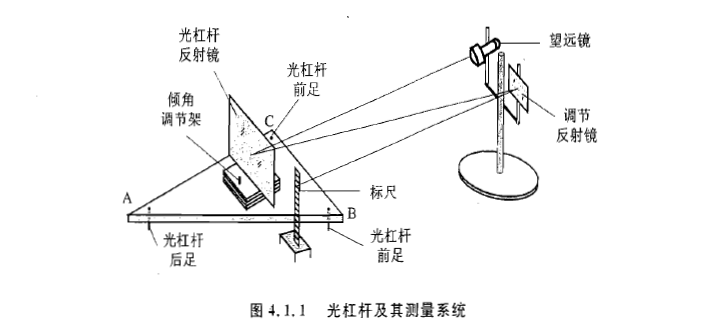
\includegraphics[width=12cm]{Image/光杠杆及其测量系统.png}
\end{figure}
光杠杆的结构如图4.1.1所示。
开始时光杠杆反射镜与标尺在同一平面,在望远镜上读到的标尺读数为$r_0$,当光杠杆反射镜的后足尖下降$\delta L$时,产生一个微小的偏角$\theta $,在望远镜上读到的标尺读数为$r_{i}$,则放大后的钢丝伸长量$C_{i}=r_i-r_0$。由图4.1.2可知
$$ \delta L_i=b\cdot \tan \theta \approx b\theta $$
式中,b为光杠杆前后足间的垂直距离,称光杠杆常数。
\begin{figure}[H]
\centering
  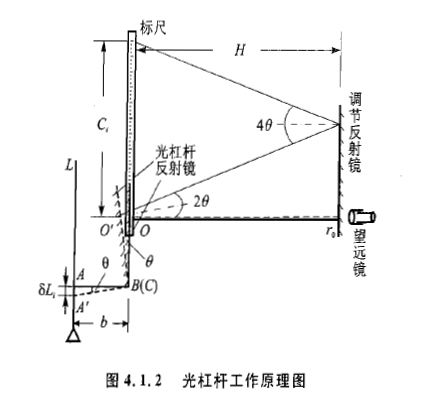
\includegraphics[width=7cm]{Image/光杠杆工作原理图.png}
\end{figure}
由于经光杠杆反射而进入望远镜的光线方向不变,故当平面镜旋转一定角度$\theta$之后,入射到光杠杆的光线方向就要偏转$4\theta$,因$\theta$甚小,OO'也甚小,故可认为平面镜到标尺的距离$H\approx O'r_0$,并有
\begin{center}
$2\theta \approx \tan 2\theta = \displaystyle\frac{C_i/2}{H},\theta =\displaystyle\frac{C_i}{4H}$
\end{center}
因此有
\begin{center}
$\delta L_i=\displaystyle\frac{bC_i}{4H}=WC_i,W=\displaystyle\frac{b}{4H}$
\end{center}
代入可得:

$$ E=\displaystyle\frac{16FLH}{\pi D^2bC_i}$$

\subsection*{实验2.扭摆法测转动惯量}
扭摆在其垂直轴l上装有一根薄片状的螺旋弹簧,用以产生恢复力矩。在轴的上方可以装上各种待测物体。将物体在水平面内转过一角度$\theta$后,在弹簧的恢复力矩作用下,物体就开始绕垂直轴作往返扭转运动。根据胡克定律,弹簧受扭转而产生的恢复力矩M与所转过的角度$\theta$成正比,即
\begin{center}
$M=-K\theta$
\end{center}
式中,K为弹簧的扭转常数。根据转动定律M总=Iβ(I为物体绕转轴的转动惯量,β为角加速度),忽略轴承的摩擦阻力矩,则有M总=M。由$\beta = \ddot{\theta}$,并令$\omega ^2=\displaystyle\frac{K}{I}$,得
\begin{center}
$\beta =\displaystyle\frac{d^2\theta}{dt^2}=-\displaystyle\frac{K}{I}\theta=-\omega ^2\theta $
\end{center}
上述方程表示扭摆运动具有角谐振动的特性:角加速度与角位移成正比,且方向相反。此方程的解为
\begin{center}
$\theta =A\cos (\omega t+\varphi )$
\end{center}
式中,A为谐振动的角振幅,$\varphi$为初相位角,$\omega$为角(圆)频率。此谐振动的周期为
\begin{center}
$ T=\displaystyle\frac{2\pi }{\omega}=2\pi \sqrt{\displaystyle\frac{I}{K}}$
\end{center}
利用上式,测得扭摆的摆动周期后,在I和K中任何一个量已知时即可计算出另一个量。

本实验用一个几何形状规则的物体(圆柱),其转动惯量($I_1$)可以根据它的质量和几何尺寸用理论公式直接计算得到,再算出本仪器弹簧的K值。若要测定其他形状物体的转动惯量,只需将待测物体安放在本仪器顶部的各种夹具上,测定其摆动周期,由上式即可换算出该物体绕转动轴的转动惯量。理论分析证明,若质量为m的物体绕过质心轴的转动惯量为$I_c$,当转轴平行移动距离x时,则此物体对新轴线的转动惯量变为$I_c+mx^2$。这称为转动惯量的平行轴定理。




\section*{三、实验仪器}
细钢丝、光杠杆、望远镜、标尺、拉力测量装置、钢卷尺、游标卡尺、螺旋测微器、扭摆、塑料圆柱体、金属空心圆筒、实心塑料(或木)球、金属细长杆(两个滑块可在上面自由移动)、数字式计时器、电子天平;三线摆、钢卷尺、电子秒表、圆环、气泡水平仪。

\section*{四、实验步骤}
\subsection*{实验1.拉伸法测钢丝弹性模量}
\subsubsection*{(1)调整测量系统}
\begin{enumerate}
\item 目测粗调
\item 调焦找尺
\item 细调光路水平
\end{enumerate}
\subsubsection*{(2)测量数据}
\begin{enumerate}
\item 首先预加10kg拉力,将钢丝拉直,然后逐次改变钢丝拉力,测量望远镜水平叉丝对应的标尺读数。
\item 根据量程及相对不确定度大小,选择合适的长度测量仪器,分别用卷尺、游标卡尺或千分尺测L、H、b各一次,测钢丝直径D若干次。
\end{enumerate}
\subsubsection*{(3)数据处理}
选择用逐差法、一元线性回归法或图解法计算弹性模量并估算不确定度。
\begin{enumerate}
\item L的误差限为0.3cm
\item H的误差限为0.5cm
\item b的误差限为0.02cm
\end{enumerate}

\subsection*{实验2.扭摆法测转动惯量}
\subsubsection*{(1)调整测量系统}
用水准仪调整仪器水平,设置计时器。
\subsubsection*{(2)测量数据}
\begin{enumerate}
\item 装上金属载物盘,测定其摆动周期$T_0$;将塑料圆柱体垂直放在载物盘上,测出摆动周期$T_1$,测定扭摆的弹簧扭转常数K。
\item 测定金属圆筒、塑料(或木)球与金属细长杆的转动惯量。列表时注意给出各待测物体转动惯量的测量公式(金属圆筒$I_2$、塑料球$I_3$以及金属细长杆$I_4$)和理论计算公式(金属圆筒$J_2$、塑料球$J_3$ 以及金属细长杆$J_4$)。
\item 验证转动惯量平行轴定理。将滑块对称地放置在细杆两边的凹槽内(此时滑块质心离转轴的距离分别为5.00、10.00、15.00、20.00、25.00(单位:cm))测出摆动周期$T_5i$。若时间许可,还可以将两个滑块不对称放置(例如分别取5.00与10.00,10.00与15.00,
15.00与20.00,20.00与25.00(单位:cm)),这样采用图解法验证此定理时效果更好。
\item 测量其他常数。利用电子天平,测出塑料圆柱、金属圆筒、塑料(或木)球与金属细长杆的质量,并记录有关物体的内、外径和长度。
\end{enumerate}
\subsubsection*{(3)数据处理}
\begin{enumerate}
\item 设计原始数据记录表格;
\item 算出金属圆筒、塑料(或木)球和金属细长杆的转动惯量$I_2$、$I_3$、$I_4$,并与理论计算值$J_2$、$J_3$、$J_4$比较,求百分差;
\item 验证平行轴定理。
\end{enumerate}

\end{document}